\documentclass{standalone}
\usepackage[english]{babel}
\usepackage[utf8x]{inputenc}
\usepackage{pgfplotstable}
\usepackage{pgfplots}
\usepackage{tabularx}
\usepackage{multirow}
\usepackage{booktabs}
\usepackage{tikz}

\usetikzlibrary{arrows,shapes,chains,positioning,scopes}
\usetikzlibrary{fit,calc,backgrounds,patterns}
\usetikzlibrary{shadows}

% \tikzstyle{decision} = [diamond, draw, fill=blue!20,aspect=2, 
%     text width=4.5em, text badly centered, node distance=1.75cm, inner sep=0pt]
    
\tikzstyle{localnode}    = [rectangle, draw, fill=gray!20, 
    text width=5em, text centered, rounded corners, minimum height=4em,node distance=3.5cm]
\tikzstyle{servernode} = [rectangle, draw, fill=green!20, 
    text width=5em, text centered, rounded corners, minimum height=4em,node distance=3.5cm]
    
% \tikzstyle{localnode} = [rectangle, draw, fill=green!20, 
%     text width=5em, text centered, rounded corners, minimum height=4em,node distance=3.5cm]
    
\tikzstyle{line} = [draw, -latex']
\tikzstyle{cloud} = [draw, ellipse,fill=red!20, node distance=2.5cm,
    minimum height=2em]
   
        
\usetikzlibrary{arrows}    
\begin{document}    

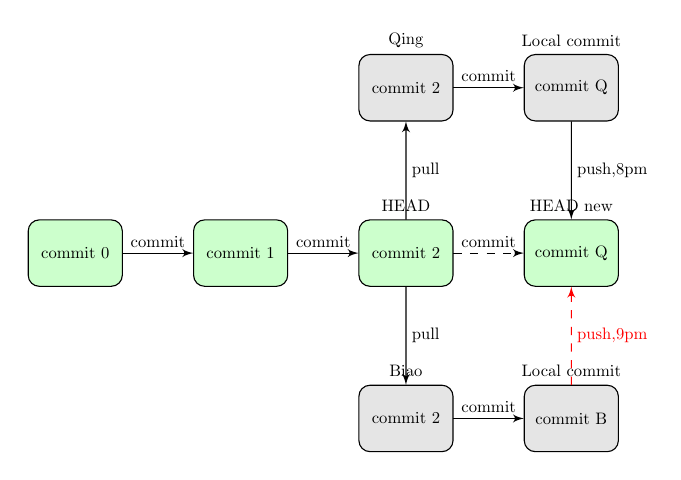
\begin{tikzpicture}[xscale=.15,yscale=.5, every node/.style={scale=.6}]
    % Place nodes

    \node [servernode]                        (workingCode0) {commit 0}; \node [above of=workingCode0] (above0)  {};
    \node [servernode, right of=workingCode0] (workingCode1) {commit 1}; \node [above of=workingCode1] (above1)  {};    
    \node [servernode, right of=workingCode1] (workingCode2) {commit 2}; \node [above of=workingCode2] (above2)  {HEAD};
    
    \node [localnode, above of=workingCode2] (workingCodeQ) {commit 2}; \node [above of=workingCodeQ] (aboveQ)  {Qing}; 
    \node [localnode, right of=workingCodeQ] (workingCodeQ0) {commit Q};\node [above of=workingCodeQ0] (aboveQ0) {Local commit}; 
    
    \node [localnode, below of=workingCode2] (workingCodeB) {commit 2}; \node [above of=workingCodeB] (aboveQ)  {Biao};
    \node [localnode, right of=workingCodeB] (workingCodeB0) {commit B}; \node [above of=workingCodeB0] (aboveQ)  {Local commit};
    
    \node [servernode, right of=workingCode2] (workingCode3) {commit Q}; \node [above of=workingCode3] (above3)  {HEAD new};
    


    \path [line] (workingCode0) -- node [above]{commit} (workingCode1);
    \path [line] (workingCode1) -- node [above]{commit} (workingCode2);
    \path [line, dashed] (workingCode2) -- node [above]{commit} (workingCode3);    
    
    \path [line] (workingCode2) -- node [right]{pull} (workingCodeQ);    
    \path [line] (workingCodeQ) -- node [above]{commit} (workingCodeQ0);    
    \path [line] (workingCodeQ0) -- node [right]{push,8pm} (workingCode3);    

    \path [line] (workingCode2) -- node [right]{pull} (workingCodeB);    
    \path [line] (workingCodeB) -- node [above]{commit} (workingCodeB0);    
    \path [line, dashed, red] (workingCodeB0) -- node [right]{push,9pm} (workingCode3);        
%     \path [line] (Bs)    -- node [left]{Yes} (Cond1);
%     \path [line] (Cond1) -- node [left]{Yes} (Cond234);    
%     \path [line] (PUorTU) -- node [above]{No} (Exit);    
%     \path [line] (Bs)     -| node [right]{No} (Exit);
%     \path [line] (Cond1)  -| node [right]{No} (Exit);
%     
%     \path [line] (Bs)     --                     (BsEnd);    
%     \path [line] (Cond1)  --                  (Cond1End);
% 
%     
%     \node [below of=Cond234,node distance=1cm] (Cond234End) {};
%     \node [cloud, left  of=Cond234End,node distance=3cm] (SF) {strong : 3 pels};
%     \node [cloud, right of=Cond234End,node distance=3.75cm] (NF) {normal : 1 or 2 pels};
%     
%     \path [line] (Cond234)  |-node [above left]{Yes}  (SF);
%     \path [line] (Cond234)  |-node [above right]{No}  (NF);
    


    
%     \node [rectangle, right of=Exit, node distance=3cm, minimum width=3cm] (Explanation) {Cond1,2,3,4: \n decided by the red samples};
%     \path [line] (Cond234) -| node [near start] {No} (Exit);
% %     \path [line] (update) |- (Bs);
%     \path [line] (Cond234) -- node {no}(stop);
%     \path [line,dashed] (expert) -- (PUorTU);
%     \path [line,dashed] (system) -- (PUorTU);
%     \path [line,dashed] (system) |- (Cond1);
\end{tikzpicture}
\end{document}

